\section{Quarkonium production}

Measurements of quarkonium production promise to yield important information about the 
strongly-interacting system formed in heavy-ion collisions.  The in-medium dissociation of quarkonium states
in these collisions is expect to reflect both the states binding energy as 
well as the temperature of the medium, leading to a sequential suppression or disappearance
of the various charmonium and bottomonium states~\cite{Matsui:1986dk,Digal:2001ue}.
A J/$\psi$ suppression was also observed at RHIC, in central Au-Au collisions~\cite{Adare:2006ns,Adare:2011yf},

J/$\psi$ production in heavy-ion collisions has been studied over a wide range of 
collisions energies at the CERN SPS and RHIC, with a strong suppression of \jpsi
yields observed in central collisions for $rootsNN \approx 20$ to $200$~GeV.
The interpretation of the observed suppression is complicated by the presence 
of Cold Nuclear Matter effects such as nuclear absorption and (anti-) shadowing. A quantitative
description furthermore needs to take into account feeddown from excited states, 
which contribute a significant fraction of the inclusive \jpsi yield in \pp collisions.
Finally, and perhaps most importantly, the large abundance of deconfined charm quarks 
at RHIC and higher energies requires the consideration of a recombination component 
in addition to direct \jpsi production, which may mask the suppression of the initial 
\jpsi formation~\cite{{BraunMunzinger:2000px},{Thews:2000rj},{Andronic:2007bi},{Zhao:2007hh}}.

The large increase in the charm cross-section at LHC should magnify these regeneration 
effects compared to lower energy collisions, and thus provide the opportunity to disentangle
suppression and regeneration effects in a study of the energy and transverse momentum dependence
of \jpsi production. 

The LHC collision energies also facilitate high statistics studies of the \PgU family, where 
the three \PgUn states are connected by the common initial bottom pair production and 
similar kinematics, but distinguished by the hierarchy of their binding energies. In an 
in-medium dissociation picture, one therefore expects a distinct pattern in the suppression
of the \PgUn states.

\subsection{Charmonium suppression in PbPb collisons}

J/$\psi$ production in \PbPb\ collisions can be characterized by the relative to the \Ncoll scaled reference 
distributions by the \Rcp and \Raa nuclear modification factors introduced earlier.
A strong suppression of high-\pt inclusive \jpsi in the dimuon decay channel was observed in central \PbPb\ collisions
at $\rootsNN = 2.76$ TeV  relative to peripheral \PbPb\ collisions by ATLAS.
~\cite{Aad:2010aa} and with respect to \pp collisions by CMS~\cite{Chatrchyan:2012np}.

Results for the suppression of low \pt \jpsi production from ALICE are shown 
in Fig.~\ref{fig:GR:raavsy} for $\pt > 0$\GeVc (square markers) and 
$\pt > 3$\GeVc (diamond markers). and . Also shown in the plot are CMS data~\cite{Chatrchyan:2012np} 
for rapdity $ 1.6 < |y| < 2.4 $ and $\pt > 3$\GeVc. 

\begin{figure}
\begin{center}
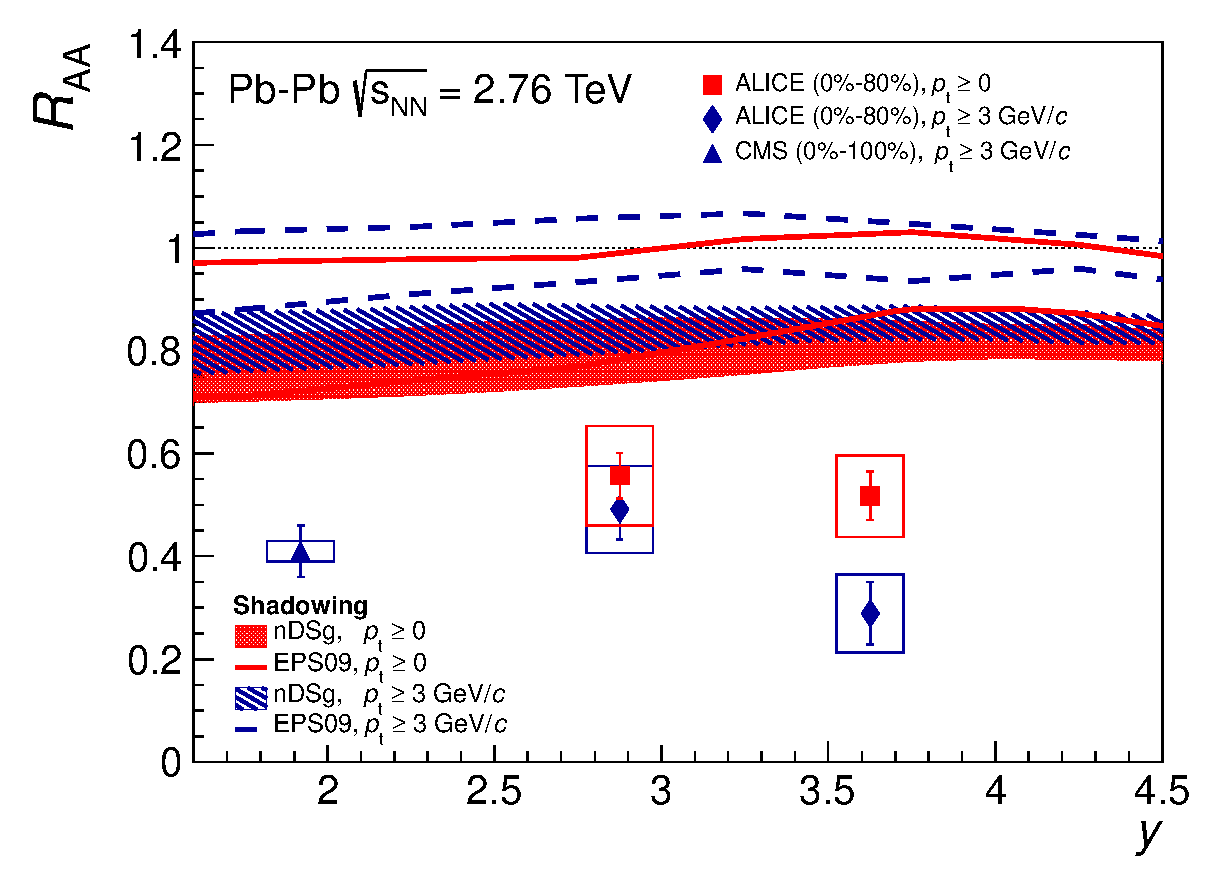
\includegraphics[width=0.49\linewidth]{qqbarfigures/RAAvsY_v7.eps}
\caption{ \label{fig:GR:raavsy}  Centrality integrated inclusive J/$\psi$ $R_{\rm{AA}}$ measured in Pb-Pb
collisions at $\sqrt{s_{\mathrm{NN}}} = 2.76$ TeV as a function of  rapidity  for two $p_{\rm{t}}$ ranges.
The open boxes contain the total systematic uncertainties except the ones on the integrated luminosity in the pp reference
 and on the $T_{\rm{AA}}$, i.e.  5.2\% (8.3\%) for the  ALICE (CMS~\cite{Chatrchyan:2012np}) data.
The two models~\cite{Ferreiro:2011rw,Vogt:2010aa} predict the  $R_{\rm{AA}}$  due  only to shadowing effects
for  nDSg (shaded areas) and EPS09 (lines) nPDF respectively.}
\end{center}
\end{figure}

Within uncertainties, neither \pt range shows a strong dependence of \jpsi\ suppression on rapidity. 
The suppression is stronger than expected for shadowing effects in the Color Singlet Model
~\cite{Ferreiro:2011rw} and the Color Evaporation Model~\cite{Vogt:2010aa}. Neither model
predicts a strong rapidity dependence.

A stronger initial state suppression has been predicted in the Color Glass Condensate (CGC) model ~\cite{Dominguez:2011cy}, 
predicting  \jpsi\ $\Raa \approx 0.5$. This prediction can be confronted with the \pt\ dependence
of \jpsi\ suppression, with initial state suppression models leading to a stronger suppression at lower \pt.
In contrast, possible \jpsi\ regeneration effects in statistical hadronization~\cite{{BraunMunzinger:2000px, Thews:2000rj}} 
and partonic transport~\cite{{Zhao:2007hh},{Liu:2009nb}} models are expected to enhance  
\jpsi\ yields at low \pt\ due to the higher phase space density of charm quarks at lower \pt.

Data from ALICE and CMS on the \pt\ dependence of the \jpsi\ \Raa\ integrated over a wide range of \PbPb\ collision centrality
is shown in Fig.~\ref{fig:GR:raaexp2}. Although the two sets cover different rapidity ranges ($2.0 < |\y| < 4.0$ vs $ 1.6  < |\y| < 2.4 $)
a common, strong \pt\ evolution of \jpsi\ \Raa\ is seen, ranging from $\approx 0.8$ at low \pt\ to $\approx 0.4$ for $\pt > 5$\GeVc.
This observation clearly favors models including a low-\pt enhancement due to charm recombination.

An even more striking observation is shown in the bottom panel of Fig.~\ref{fig:GR:raaexp2}, which compares 
the ALICE forward-rapidity \jpsi\ \Raa\ for 0\%--20\% central \PbPb\ collisions at  $\rootsNN = 2.76$\TeV 
with central \AuAu\ data from PHENIX at $\rootsNN = 0.2$\GeV and rapidity $1.2 < |\y| < 2.2$~\cite{Adare:2011yf}.
At low \pt\ the ALICE \Raa\ is about four times larger than that seen at the lower energy, while 
at the same time the initial energy density of the system at LHC is estimated to be larger than at 
RHIC by a similar factor. While a quantative interpretation of this result will require 
a detailed understanding of CNM effects at the two energies, the results are qualitatively consistent 
with the collision energy trend expected in recombination approaches such as
\cite{Zhao:2007hh,Zhou:2013aea,Liu:2009nb}.
First results of \jpsi\ production in \pPb\ collisions at the LHC have recently been presented~\cite{Abelev:2013yxa,Aaij:2013zxa}, allowing
the calibration of CNM effects vs final state suppression and recombination.

%--------------------------------------------------
\begin{figure}[h!]
\begin{center}
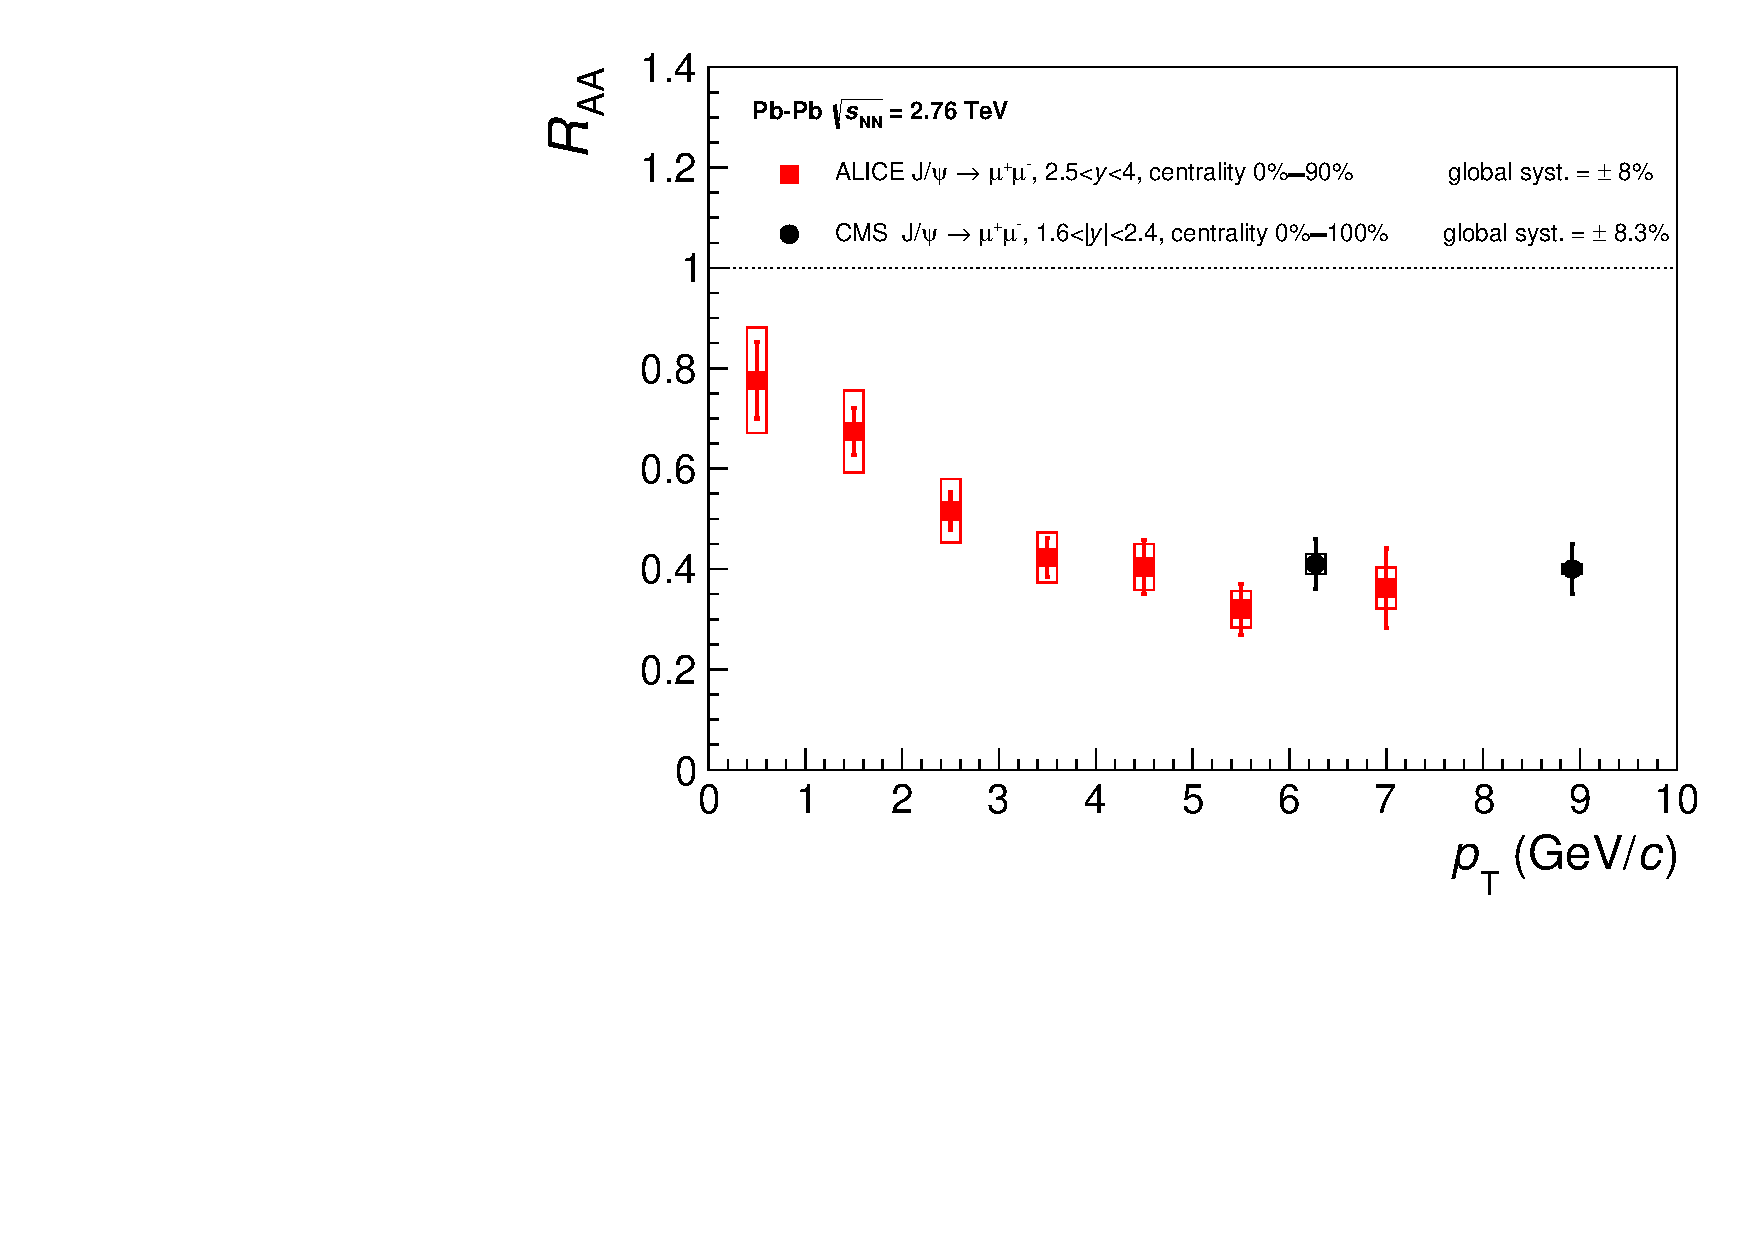
\includegraphics[width=0.49\linewidth,keepaspectratio]{qqbarfigures/RAAPtvsModels1.pdf}
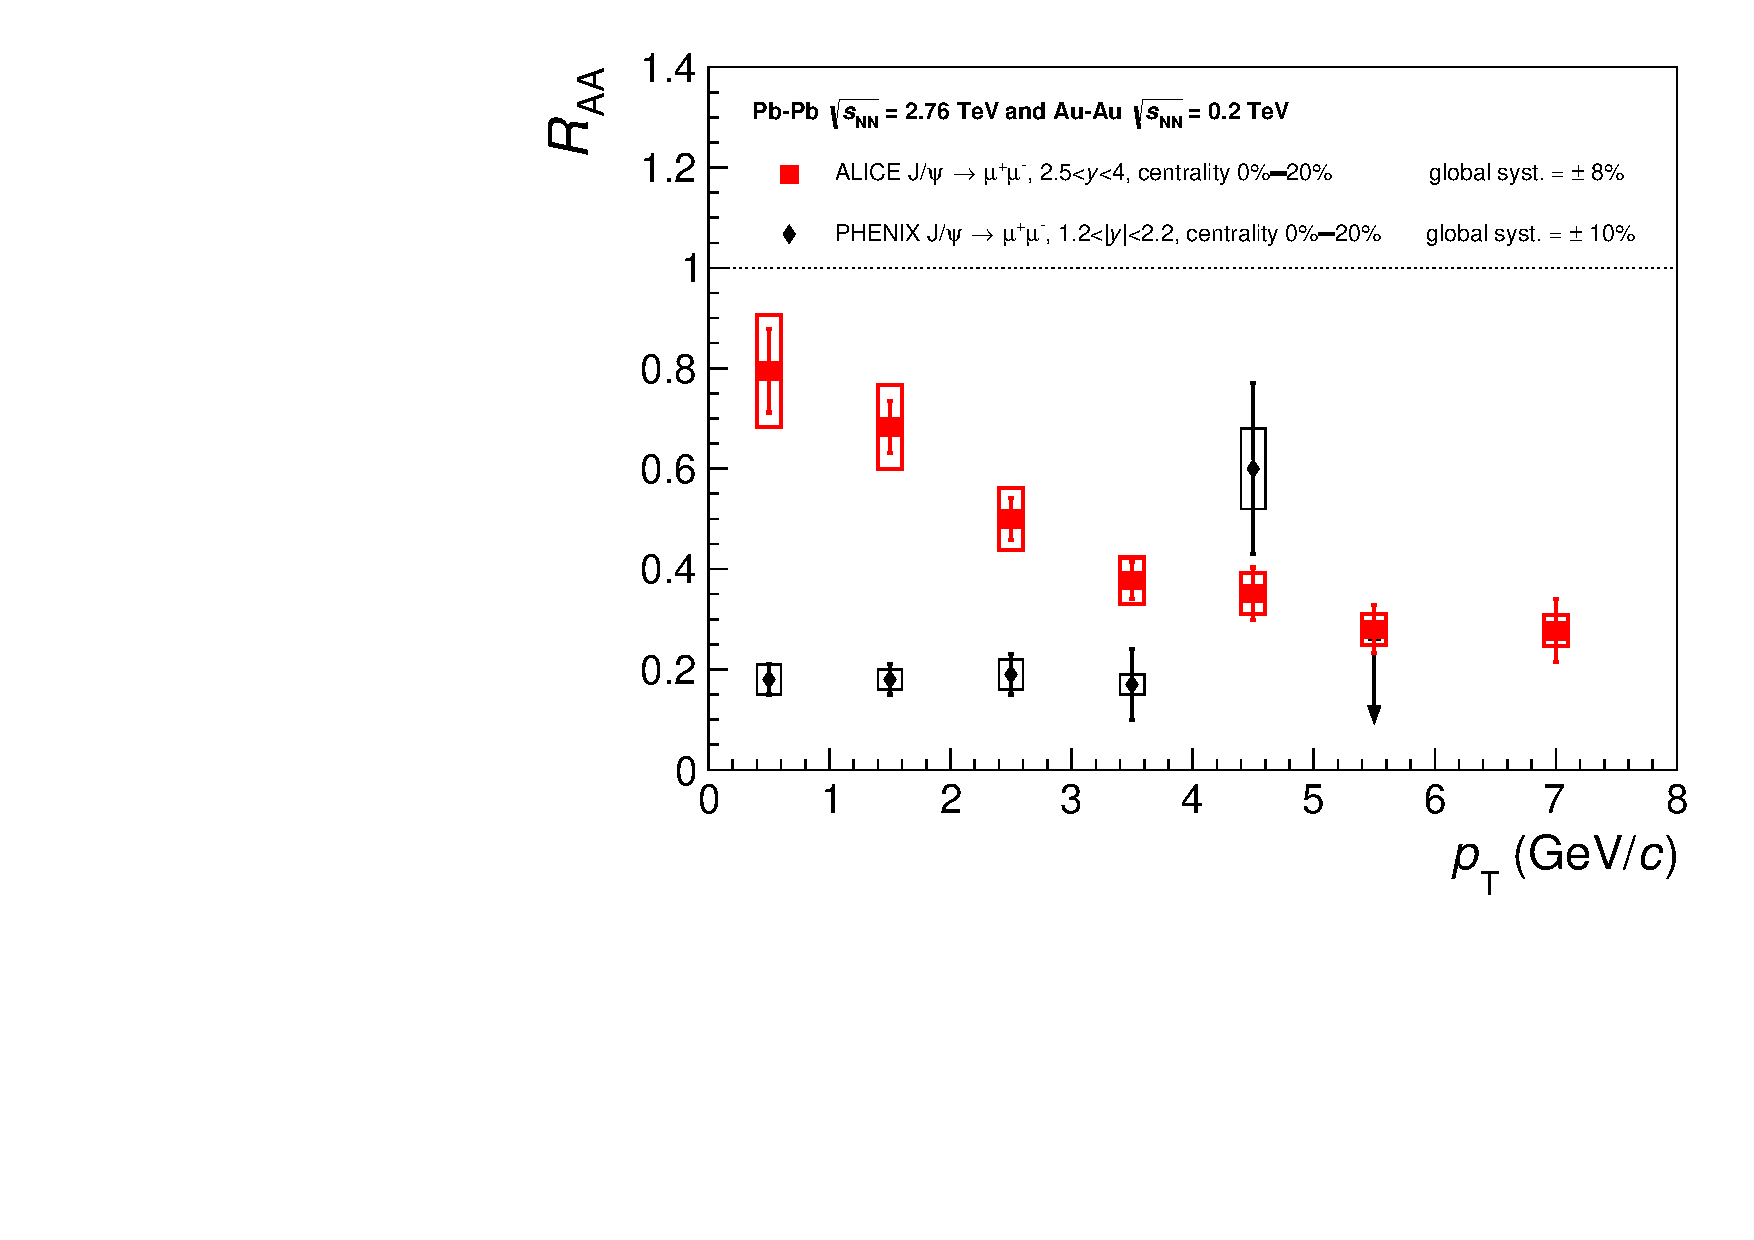
\includegraphics[width=0.49\linewidth,keepaspectratio]{qqbarfigures/RAAPtvsModels2.pdf}
\caption{ \label{fig:GR:raaexp2}
(Top):Transverse momentum dependence of the centrality integrated \jpsi\ \Raa\ measured by ALICE in \PbPb\ collisions at $\rootsNN = 2.76$\TeV compared to CMS~\cite{Chatrchyan:2012np} results at the same energy.
(Bottom): transverse momentum dependence of the \jpsi\ \Raa\ measured by ALICE in the 0\%--20\% most central \PbPb\ collisions at 2.76\TeV compared to PHENIX~\cite{Adare:2011yf} results in the 0\%--20\% most central \AuAu\ collisions at 200\GeV.}
\end{center}
\end{figure}


\subsection{Charmonium elliptic flow}

An important question for models implementing the competing contributions of 
\jpsi\ dissociation in the medium and \jpsi\ regeneration via charm quark recombination is 
the degree of charm quark thermalization. The question of thermalization in heavy-ion collisions is typically addressed
via studies of hydrodynamic flow. ALICE has recently presented the first data suggesting non-zero elliptic flow
in \PbPb\ collisions, providing important information on this topic.

In a dissociation/recombination type approach, elliptic flow of the observed \jpsi\ can arise from multiple 
contributions. Those \jpsi\ produced in the initial hard scattering traverse a shorter path in the medium when 
travelling in-plane vs out-of-plane, leading to a possible azimuthal modulation of \jpsi\ yields with respect
to the event plane. If the charm quarks participate in the collective expansion of the medium, as 
suggested by the observed elliptic flow of open charm mesons, \jpsi\ produced by recombination will 
pick up the elliptic flow of the charm quarks. These contributions can possibly be disentangled by 
studies of the \pt dependence of \jpsi\ suppression and \jpsi\ elliptic flow.

Measurements of the \jpsi\ elliptic flow by STAR for \AuAu\ collisions at $\rootsNN = 200$\GeV 
are consistent with zero~\cite{Adamczyk:2012pw}, altough the large uncertainties prevent strong conclusions.

\begin{figure}
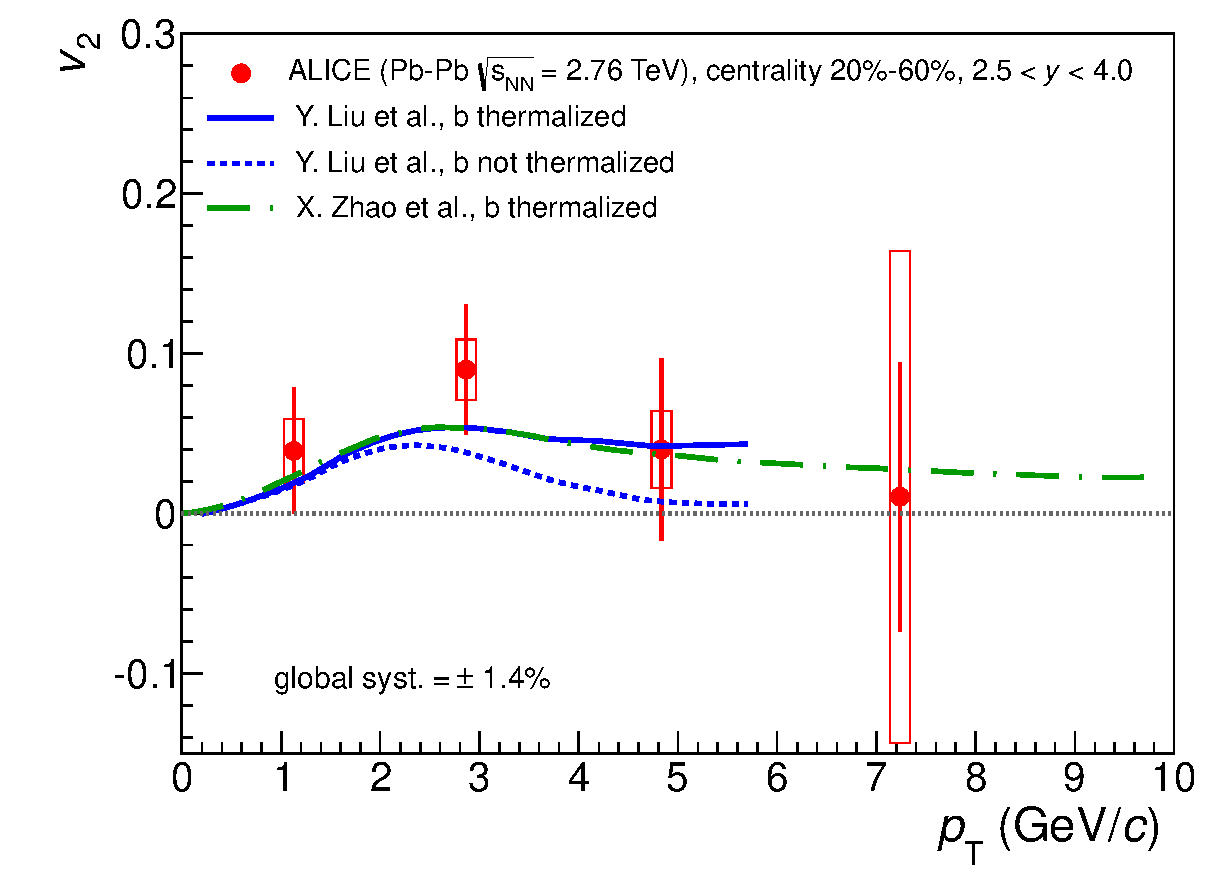
\includegraphics[width=0.49\linewidth]{qqbarfigures/prl_fig4.eps}
\caption{\label{fig:GR:v2ptcomp} Inclusive \jpsi\ \vpt  for semi-central (20\%--60\%) \PbPb\ collisions at \rootsNN~=~2.76 TeV. The \vtwo was measured in the \pt ranges: 0--2, 2--4, 4--6 and 6--10 GeV/$c$ and the points are located at the measured  $\langle p_{\rm T} \rangle^{\rm uncor}$. Calculations from two transport models~\cite{Liu:2009gx} and~\cite{Zhao:2012gc} in the same kinematic range are also shown (see text for details).}
\end{figure}

The ALICE measurement of \jpsi\ \vtwo\ as a function of transverse momentum is shown in Fig.~\ref{fig:GR:v2ptcomp} for \PbPb\ collisions
in the 20\%--60\% centrality range.
The \jpsi\ \vtwo\ data, which have a significance of about 2$\sigma$ in this centrality range, are compared to two 
transport model calculations~\cite{Liu:2009gx,Zhao:2012gc}. The models, which includes charm quark recombination effects, 
are both compatible with the data within the current large experimental uncertainties. The comparison points to the 
importance of future high statistics measurements of \jpsi\ elliptic flow at high transverse momentum ($\pt > 5$\GeVc).

In combination the \pt\ and collision energy dependence of \jpsi \Raa\ and the indication of non-zero \jpsi\ elliptic
flow suggests a significant contribution of charm quark recombination to \jpsi\ production in \PbPb\ collisions
at LHC.


\subsection{Upsilon suppression in PbPb}

Measurements by CMS have provided the first high statistics look at \PgU\ production in heavy-ion collisions.
The \PgU family, with similar decay kinematics but a large variation of binding energies, 
provides an ideal laboratory to test dissociation effects in the hot medium produced in 
heavy-ion collisions. Compared to charmonium suppression studies, uncertainties due
to CNM effects and feed-down from higher mass states are expected to be 
less important for the bottomonium family.

Dimuon invariant mass spectra in the \PgU\ mass range obtained by CMS are shown in Fig.~\ref{fig:GR:mass} for the \PbPb\ (left) 
and \pp\ (right) datasets. The data correspond to integrated luminosities of $150\mubinv$ and $230 \nbinv$ for 
\PbPb\ and \pp\, respectively. For the \pp\ data, the excellent mass resolution of the CMS muon system
allows a clear separation of the three $\PgUn$ states. A similar mass resolution is achieved for \PbPb\ collisins, 
however a strong suppression of the \PgUb\ state is evident from the from the distriution and the $\PgUc$ state 
is no longer visible above the continuum background. This is a striking visual confirmation of the expected
\PgU\ suppression pattern as a function of the \PgUn\ binding energy.

\begin{figure}[t]
\begin{center}
    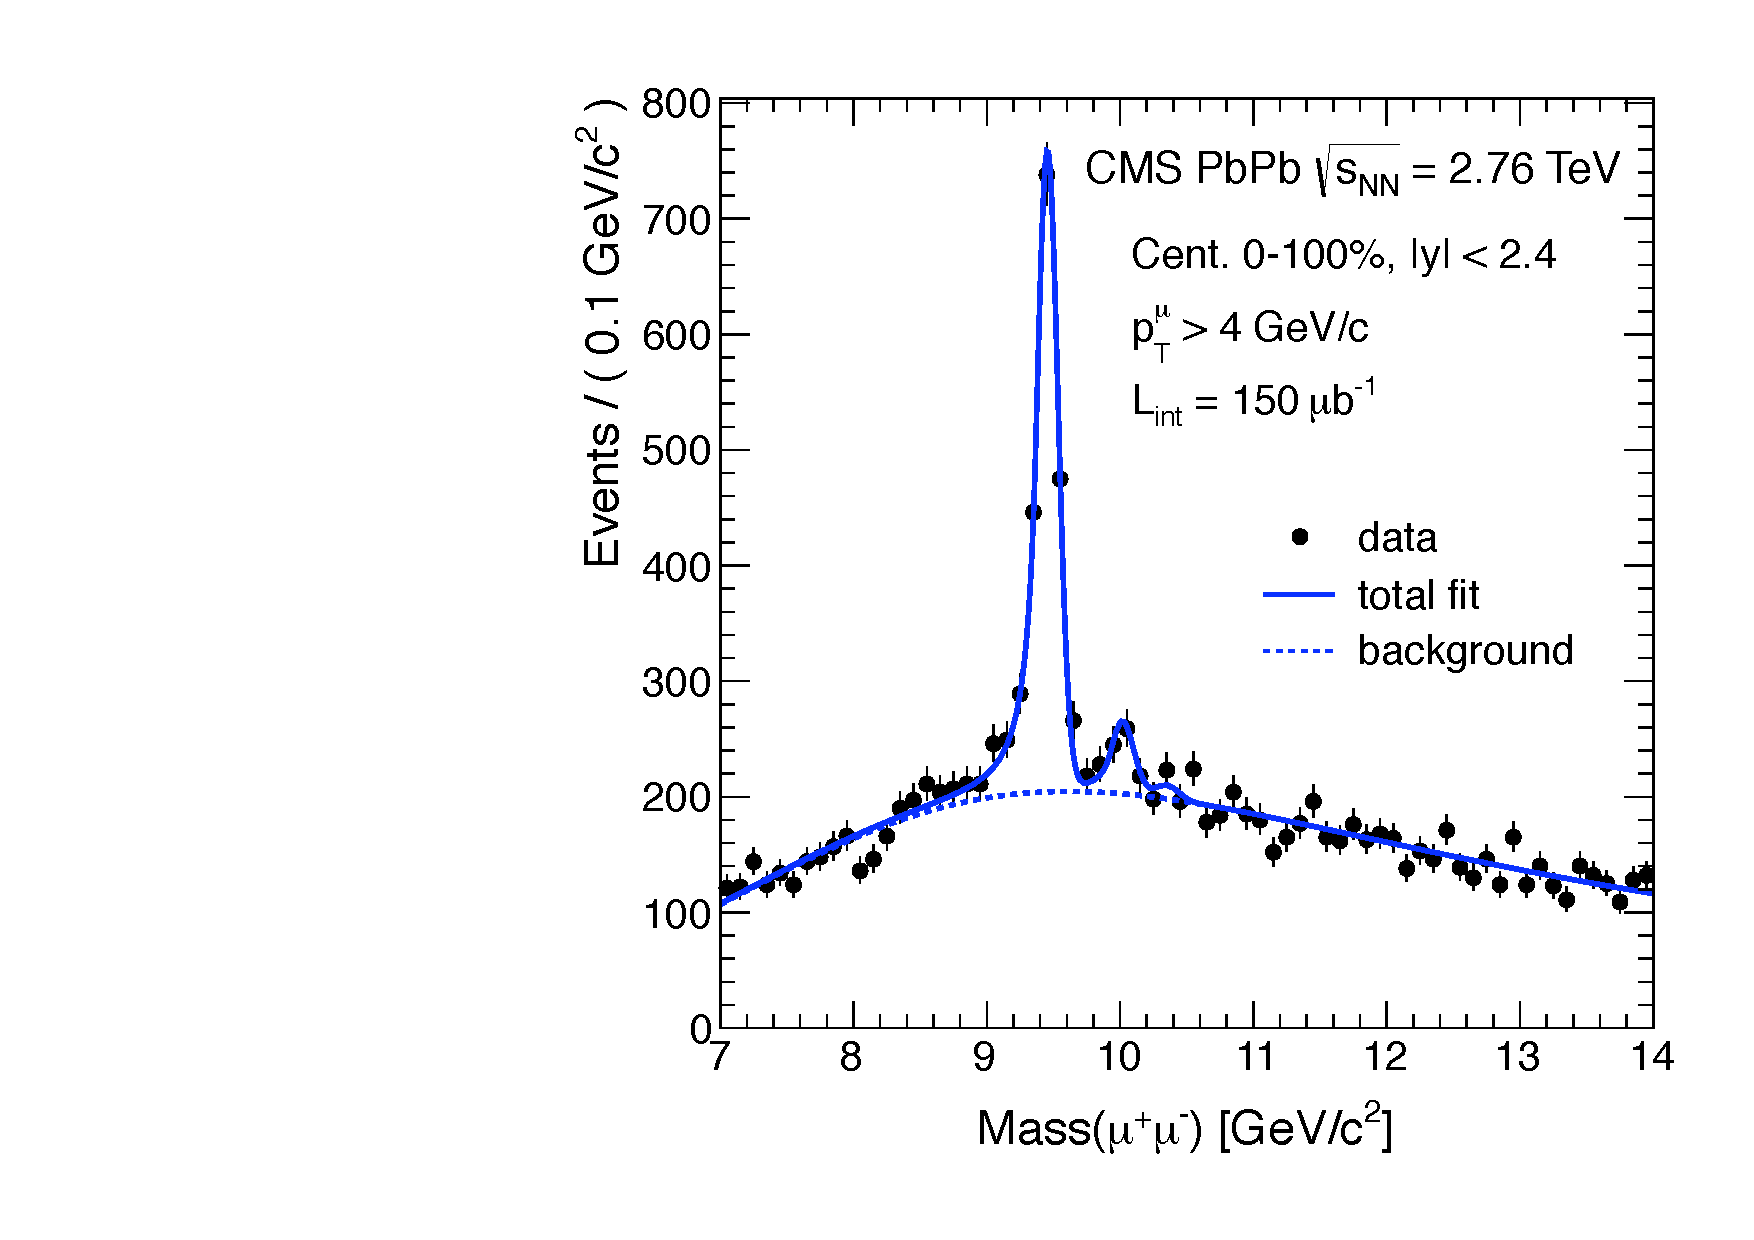
\includegraphics[width=0.45\textwidth]{qqbarfigures/hiFitPt4Erf}
    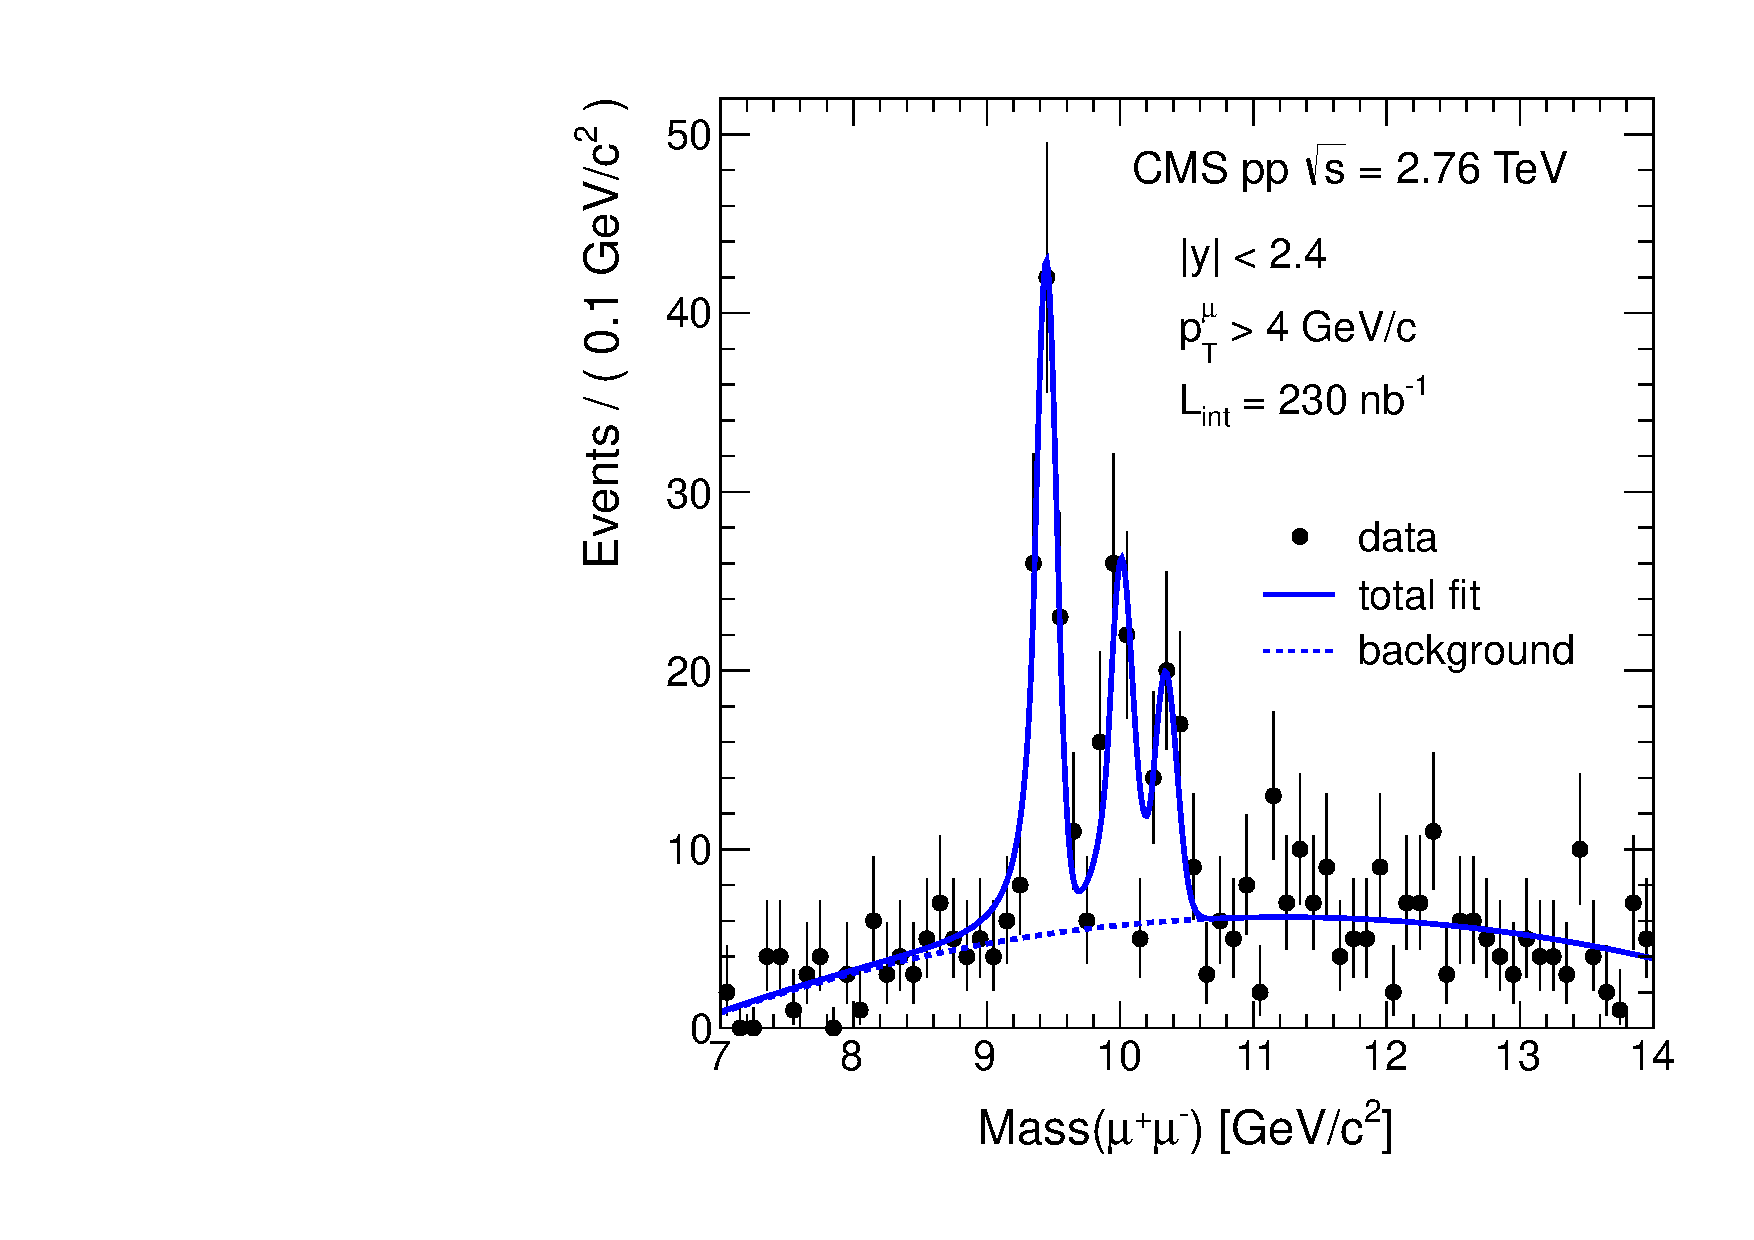
\includegraphics[width=0.45\textwidth]{qqbarfigures/ppFitPt4Erf}
    \caption{Dimuon invariant-mass distributions in \PbPb\ (left) and \pp (right)
data at $\rootsNN = 2.76$\TeV. The same reconstruction algorithm and analysis selection are applied to both datasets, including a transverse momentum requirement on single muons of $\pt > 4\GeVc$. The solid (signal + background) and dashed (background-only) curves show the results of the simultaneous fit to the two datasets.}
    \label{fig:GR:mass}
\end{center}
\end{figure}

The comparison of \pp\ and \PbPb\ data allows a characterization of the \PgU\ suppression
in terms of the nuclear modfication factor \Raa.
Integrating over centrality, the following \Raa\ values were measured for the \PgUn states:
\begin{eqnarray}
\Raa (\PgUa) &=& 0.56 \pm 0.08\,\text{(stat.)} \pm 0.07\,\text{(syst.)} \,, \\
\Raa (\PgUb) &=& 0.12 \pm 0.04\,\text{(stat.)} \pm 0.02\,\text{(syst.)} \,, \nonumber \\
\Raa (\PgUc) &=& 0.03 \pm 0.04\,\text{(stat.)} \pm 0.01\,\text{(syst.)}  \nonumber\\
\end{eqnarray}
The statistical significance of the \PgUc\ peak above the continuum is less than one standard deviation.
It should also be noted that there are significant feed-down contributions to 
the \PgUa\ state that may reach $\approx 50\%$~\cite{Affolder:1999wm, Aaij:2012se},
which opens the possibility that directly produced $\PgUa$ state are largely unsuppressed.

The \PgUa\ and \PgUb\ suppression was also studied as a function of centrality, 
as shown in Fig.~\ref{fig:GR:centrality}.
Here the relative suppression of \PgUa\ and \PgUb\ is characterized by 
the double ratio $\frac{\PgUb/\PgUa|_{\PbPb}}{\PgUb/\PgUa|_{\pp}}$ 
(Fig.~\ref{fig:GR:centrality}~(left) and the absolute suppression 
of the two states is shown as \Raa\ vs centrality (Fig.~\ref{fig:GR:centrality}~(left)).

\begin{figure}[t]
\begin{center}
   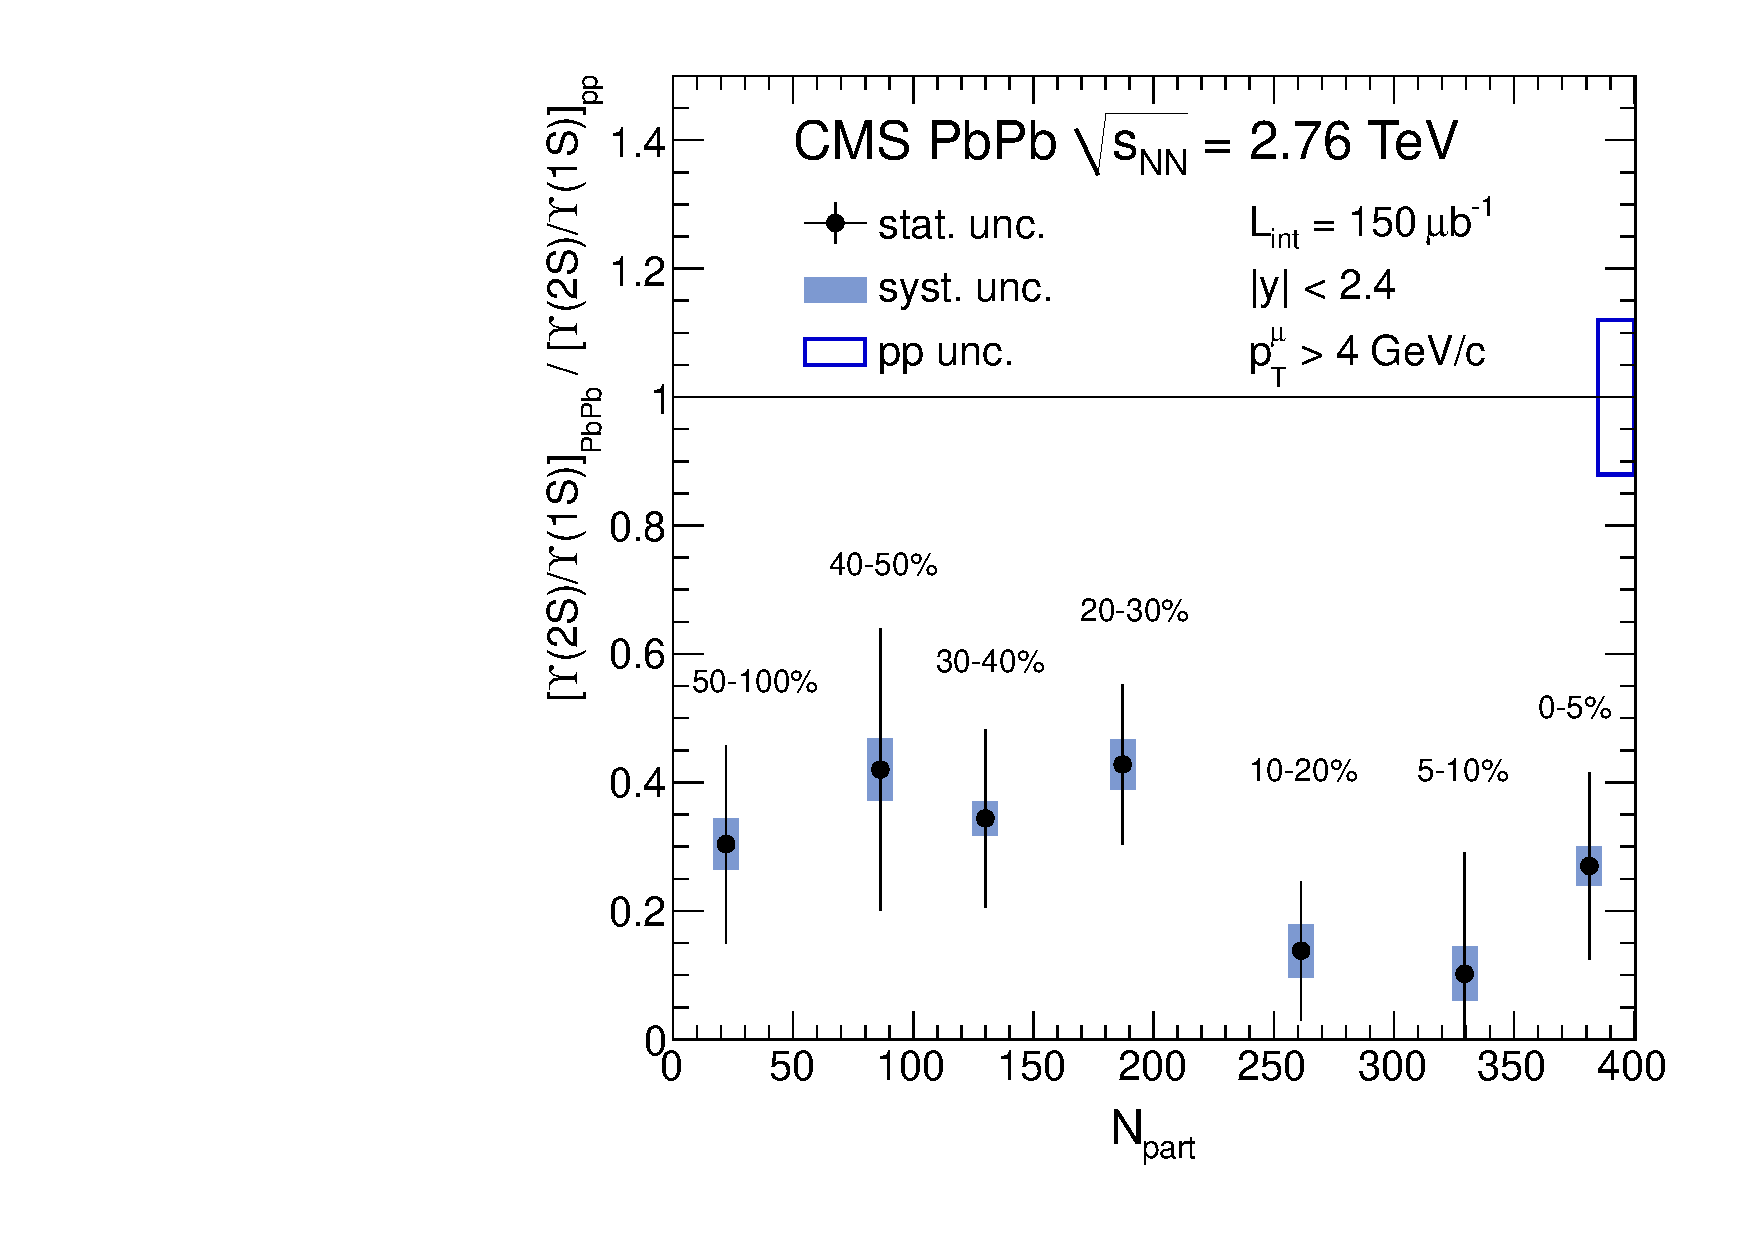
\includegraphics[width=0.45\textwidth]{qqbarfigures/chi2VsCent}
   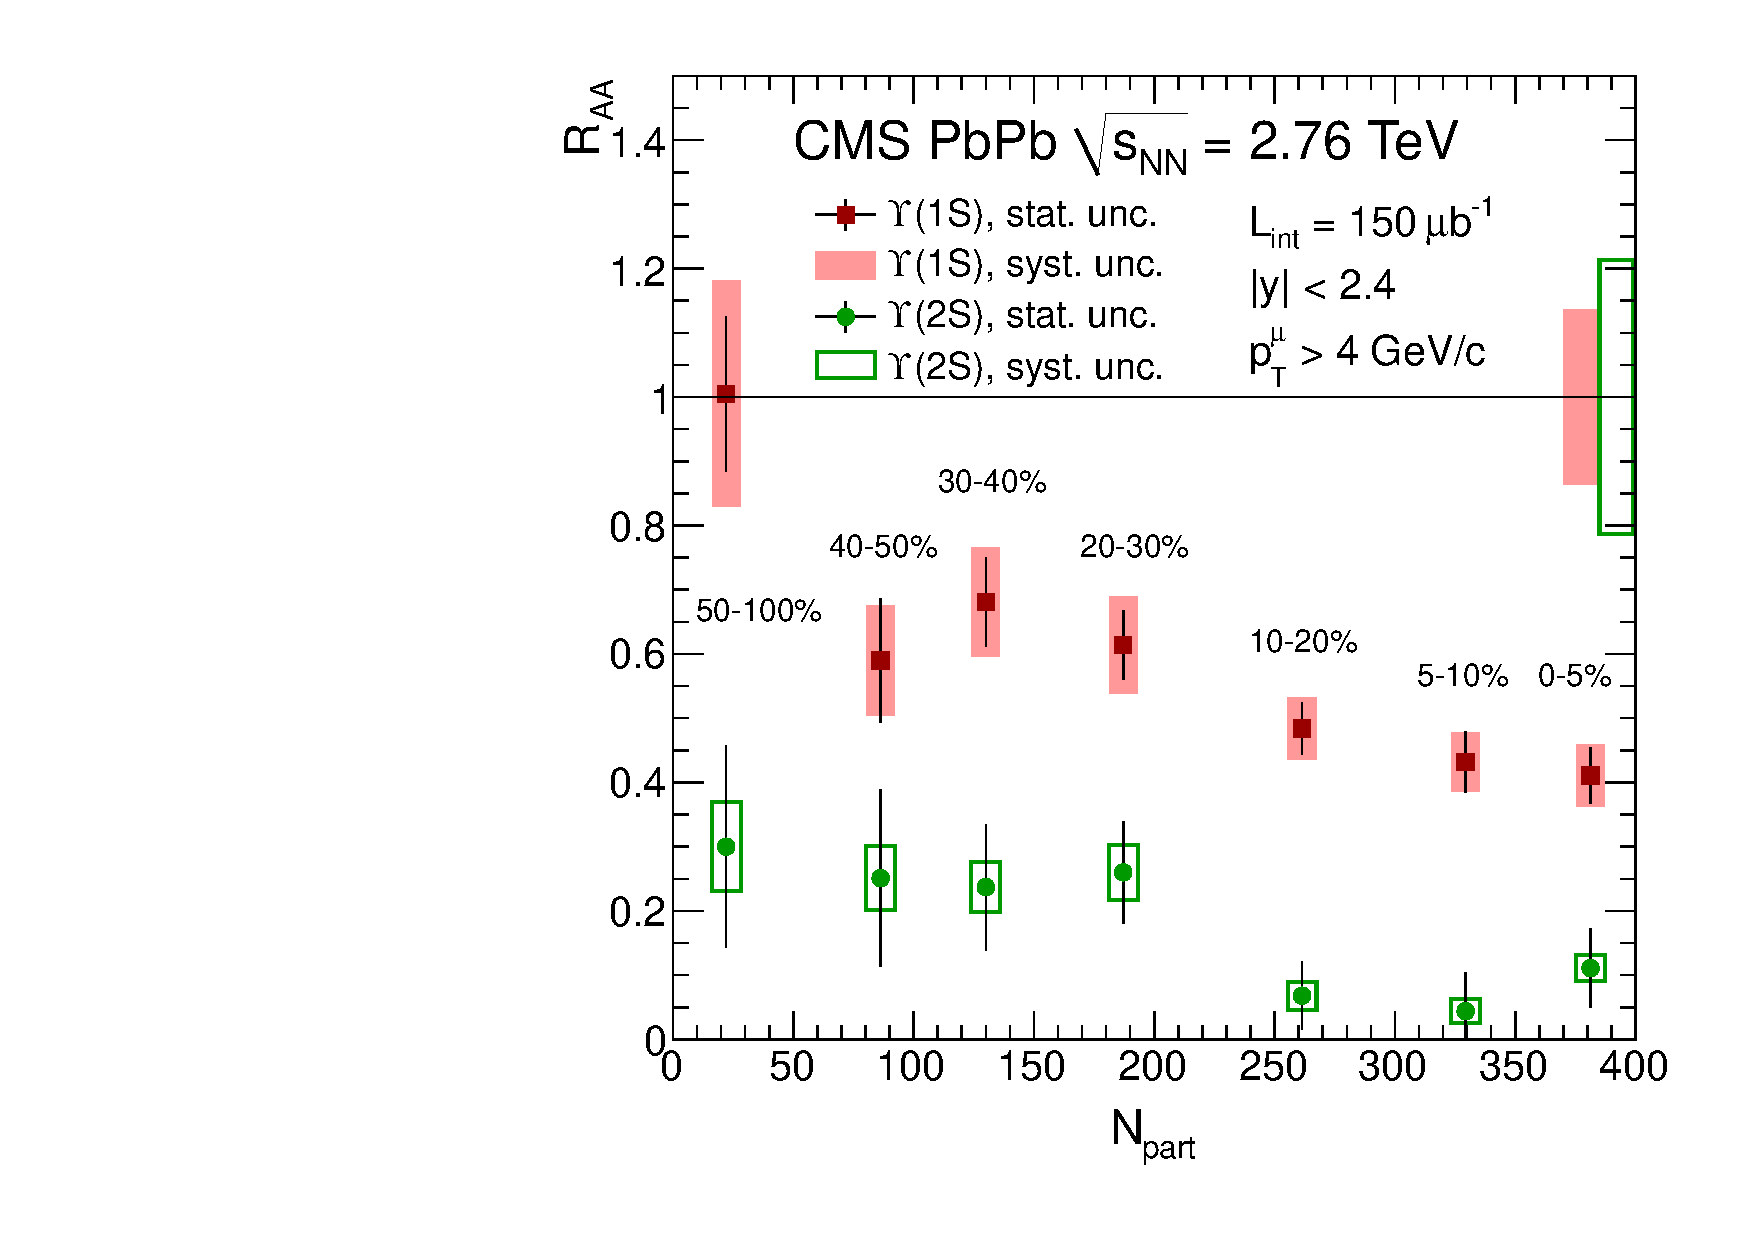
\includegraphics[width=0.45\textwidth]{qqbarfigures/RaaPt4}
  \caption{(Left) Centrality dependence of the \PgUa\ and \PgUb\ double ratios.  (Right): 
Centrality dependence of the nuclear modification factors for the $\PgUa$ and $\PgUb$ states. 
The relative uncertainties from \npart-independent quantities 
are represented by the boxes at unity, and are not included in the data points.
The event centrality bins used are indicated by percentage intervals.}
\label{fig:GR:centrality}
\end{center}
\end{figure}

While \Raa\ shows a strongly falling trend with increasing collision centrality
for both \PgUa\ and \PgUb\ (with a much stronger suppression for \PgUb), the 
double ratio does not exhibit a pronounced centrality dependence.

Overall, the data qualitatively exhibit the hierarchy in the \PgUn\ suppression pattern
expected based on the states' binding energies. Although the most peripheral bin
is rather wide (50--100\%), it is interesting observe the strong suppression of the 
\PgUb\ relative to the \PgUa\ already for this bin. Future high statistics \PbPb\ data 
should elucidate the onset of the \PgU\ suppression in the most peripheral collisions,
in combination with information on \PgU\ suppression in small systems obtained from
studies in \pPb\ reference data. 

